% used PGFPlots v1.15
\documentclass[border=5pt]{standalone}
\usepackage{pgfplots}
\usepgfplotslibrary{fillbetween}
\pgfplotsset{
    /pgf/declare function={
        % normal distribution where \mean = mean and \stddev = sd}
    gauss(\mean,\stddev) = 1/sqrt(2*pi*\stddev^2) * exp(-((\x-\mean)^2)/(2*\stddev^2));
},
    }
\begin{document}
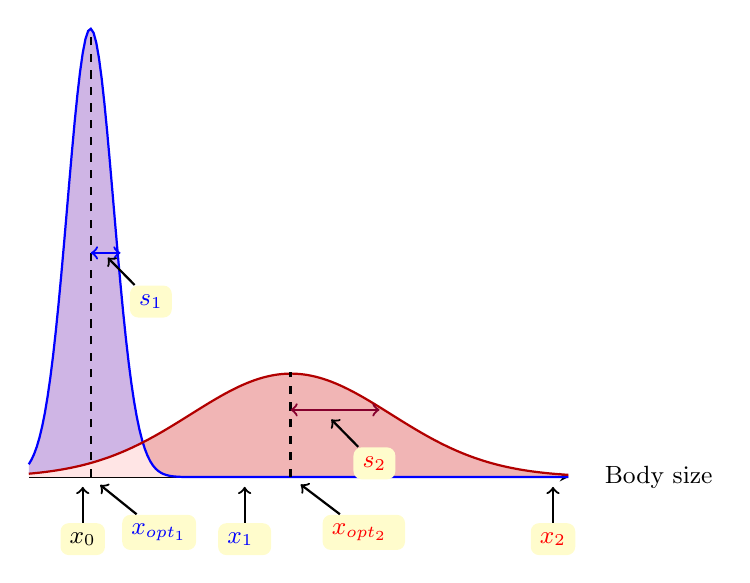
\begin{tikzpicture}[every pin edge/.style={thick,<-},
	every pin/.style={fill=yellow!20!white,rectangle,rounded corners=3pt,font=\small}]
\begin{axis}[
    axis lines=left,
    domain=0:17.5,
    samples=201,
    ymin=0,
    xtick=\empty,
    ytick=\empty,
    enlargelimits=false,
    clip=false,
	axis y line=none % enlever y axis  
]

\addplot [
    thick,
    blue,
    name path=cat,
    %fill=orange!50,
] {gauss(2, 0.75)}
%node[pos=0.3, above] {cat}
;
\addplot [
    thick,
    red!70!black,
    name path=puma,
] {gauss(8.5, 3.25)}
%node [pos=0.5, above right] {puma}
;

\path[name path=axis] (axis cs:0,0) -- (axis cs:17.5,0);

% because 'cat' and 'puma' only intersect once and both have a minimum
% value of 0, both areas can be filled with one call without filling the
% common area
\addplot[
    thick,
] fill between [
    of=cat and puma,
    split,
    every segment no 0/.style={
        fill=blue,
        fill opacity=0.25,
    },
    every segment no 1/.style={
        fill=red!70!black,
        fill opacity=0.25
    },
];

% compute + label the lower area (but do not draw it):
    \path [
     name path=lower,
     intersection segments={
         of=puma and cat,
         sequence=R1 -- L2,
     }
    ];

    % fill the lower area
    \addplot [
    fill=red!40,
        fill opacity=0.25,
    ] fill between [
        of=axis and lower,
    ];

\draw[thick,dashed] (axis description cs:0.115,0) -- (axis description cs:0.115,1); 
\draw[thick,blue,<->] (axis description cs:0.115,0.5) -- (axis description cs:0.170,0.5);
% s 
\node[pin=310:{ {\color{blue} $s_1$} }] at (axis cs:2.25,0.272) {};
\node[pin=310:{ {\color{red} $s_2$} }] at (axis cs:9.5,0.08) {};

%\draw[thick,blue,<->] (axis description cs:0.115,1) -- (axis description cs:0.485,1);
%\draw[thick,purple!70!black,<->] (axis description cs:0.485,0.3) -- (axis description cs:0.98,0.3);

% d 
%\node[pin=270:{ {\color{blue} $d_1$} }] at (axis cs:5.5,0.52) {};
%\node[pin=90:{ {\color{red} $d_2$} }] at (axis cs:12.5,0.18) {};

% x 
\node[pin=310:{{\color{blue} $x_{opt_1}$}}] at (axis cs:2,0.0) {};
\node[pin=270:{$x_{0}$}] at (axis cs:1.75,0.0) {};
\node[pin=310:{ {\color{red} $x_{opt_2}$ } }] at (axis cs:8.5,0.0) {};
\node[pin=270:{ {\color{blue} $x_{1}$ } }] at (axis cs:7,0.0) {};
\node[pin=270:{{\color{red} $x_2$} }] at (axis cs:17,0.0) {};

% phi 
% \node[]  at (axis cs:14,0.3) {$\varphi_i = (x_i,s_i,x_{opt_i})$};

\draw[thick,dashed] (axis description cs:0.485,0) -- (axis description cs:0.485,0.235); 
\draw[thick,purple!70!black,<->] (axis description cs:0.485,0.15) -- (axis description cs:0.65,0.15);
\end{axis}

\draw (8,0) node{{\small Body size}}; 

% dessiner food chain (cf git) 

%\node (1) at (7,5) {}; 
%\node (2) at (7,3.5) {}; 
%\node (3) at (7,2) {}; 
%
%\draw (7,5) node[circle,draw=black,fill=red]{2} ; 
%\draw (7,3.5) node[circle,draw=black,fill=blue] {1} ; 
%\draw (7,2) node[circle,draw=black,fill=black,text=white] {0} ; 
%
%\draw[<-] (1) to[out=180,in=180] (3) ; 
%\draw[<-,very thick] (2) to[out=0,in=0] (3) ; 
%\draw[<-,very thick] (1) to[out=0,in=0] (2) ; 


\end{tikzpicture}
\end{document}
